\documentclass[10pt,twocolumn,a4paper]{article}

\usepackage{cvpr}
\usepackage{times}
\usepackage{epsfig}
\usepackage{graphicx}
\usepackage{amsmath}
\usepackage{amssymb}
\usepackage{subfig}

\usepackage{dsfont}

% Include other packages here, before hyperref.

% If you comment hyperref and then uncomment it, you should delete
% egpaper.aux before re-running latex.  (Or just hit 'q' on the first latex
% run, let it finish, and you should be clear).
\usepackage[breaklinks=true,bookmarks=false]{hyperref}

\cvprfinalcopy % *** Uncomment this line for the final submission

\def\cvprPaperID{****} % *** Enter the CVPR Paper ID here
\def\httilde{\mbox{\tt\raisebox{-.5ex}{\symbol{126}}}}

%\newcommand{\ie}{i.~e. }
%\newcommand{\eg}{e.~g. }
%\newcommand{\wrt}{w.~r.~t. }s
\newcommand{\iid}{i.~i.~d. }


\newcommand{\abbr}[2]{#1 (#2)}
\newcommand{\abbrpl}[2]{#1s (#2s)}

\newcommand{\jacob}[2][]{%
    \ifthenelse{\equal{#1}{}}{J_{#2}}{J_{#2}(#1)}%
}
\newcommand{\jacobian}{\jacob}

\newcommand{\expt}[2]{\IE_{#1} \left[ #2 \right]}

\newcommand{\diag}[1]{\text{diag} \left[ {#1} \right]}
\newcommand{\step}{\bs 1}


\newcommand{\IR}{\mathds{R}}
\newcommand{\IN}{\mathds{N}}
\newcommand{\IE}{\mathds{E}}
\newcommand{\IB}{\mathds{B}}
\newcommand{\IM}{\mathds{M}}

\newcommand{\tc}{\tilde c}
\newcommand{\tu}{\tilde u}
\newcommand{\tv}{\tilde v}

\newcommand{\la}{\textbf{(a)}~}
\newcommand{\lb}{\textbf{(b)}~}
\newcommand{\lc}{\textbf{(c)}~}
\newcommand{\ld}{\textbf{(d)}~}

\newcommand{\normal}{\mathcal N}
\newcommand{\bern}{\mathcal B}
\newcommand{\multi}{\mathcal M}
\newcommand{\degen}{\mathcal D}

\newcommand{\relu}[1]{(#1)^{+}}
\newcommand{\softmax}{\mathcal{s}}
\newcommand{\sigmoid}{\sigma}

\newcommand{\hx}{\hat x}
\newcommand{\tx}{\tilde x}
\newcommand{\idty}{\bs I}

\newcommand{\hX}{\hat X}
\newcommand{\tX}{\tilde X}

\newcommand{\basis}{\psi}
\newcommand{\Basis}{\Psi}
\newcommand{\measure}{\phi}
\newcommand{\Measure}{\Phi}

\newcommand{\ds}{\mathcal X}

\newcommand{\loss}{\mathcal L}

\newcommand{\dims}{\mathcal D}

\usepackage[font=small,labelfont=bf]{caption}


% Pages are numbered in submission mode, and unnumbered in camera-ready
%\ifcvprfinal\pagestyle{empty}\fi
\setcounter{page}{1}
\begin{document}

%%%%%%%%% TITLE
\title{A Deep Learning Approach to\\Compressive Sensing with Convolutional Autoencoders}

\author{Steffen Schneider\\
RWTH Aachen University\\
{\tt\small steffen.schneider@rwth-aachen.de}
}

\maketitle
%\thispagestyle{empty}

%%%%%%%%% ABSTRACT
\begin{abstract}
    Compressed sensing has proven to be an important technique in signal acquisition, especially in contexts in which sensor quality or the maximum possible duration of the measurement is limited. 
    In this report, deep learning techniques are used to improve compressive sensing in the context of image acquisition.
    In a previous approach, \cite{Mousavi2015} deployed stacked denoising autoencoders capable of reconstructing images considerably faster than conventional iterative methods.
    Apart from reviewing this approach, a possible extension using convolutional autoencoders inspired by the popular VGGnet architecture is discussed.
    Instead of learning models from scratch, a simple yet effective way for adapting available filters used in ImageNet classification is presented.
    By reformulation of the autoencoder structure in terms of a fully convolutional network, the approach by \cite{Mousavi2015} can be adapted to arbritrarly large images for efficient learning of the measurement matrix and sparsity basis.
    Suggestions on the real implementation of such as system conclude the report.
\end{abstract}

%%%%%%%%% BODY TEXT
\section{Introduction}
\abbr{Compressive Sensing}{CS}, also known as Compressed Sensing, is a technique to efficiently acquire a signal that is sparse within a certain domain.
Many signals such as diffusion data in MRI or real-world images have an underlying sparse representation \cite{Donoho2006}.

In the first part of this report, CS terminology will be introduced along with the objectives a CS algorithm should meet.
Afterwards, deep learning is introduced and denoising autoencoders are introduced from a Bayesian perspective.
It is shown that these models meet the requirements of a CS algorithm.

In the following section, the original approach used by \cite{Mousavi2015} is discussed and extended to overcome several problems the authors discussed in their paper.
The final section of this report presents some experiments using these extensions for CS on image data.

\subsection{Compressive Sensing}

A signal $x \in \IR^N$ is \emph{sparse} if a representation $s \in \IR^N$ with $K \ll N$ non-zero components can be found such that $x$ can be represented as a linear combination of these components:

\begin{equation}
    x = \sum_{k} \basis^{(k)} s^{(k)} = \Basis s
\end{equation}

Here, $\basis^{(k)}$ are basis functions, collected in a matrix $\Basis$.
Many real-world signals such as images and acoustic signals have such underlying sparse representations, usually in a wavelet domain \cite{Donoho2006}.
In the following, indices $n$ will denote positions in the time domain, while $k$ is used to denote positions in the domain of (spatial) frequencies.

Sparsity within the wavelet domain is useful for compression \emph{after} acquisition of the signal and is extensively used in compression algorithms such as \emph{JPEG} making use of discrete cosine transforms on $8 \times 8$ patches of the image, audio codecs like 
\emph{MPEG} and \emph{Vorbis} incorporating properties of human sound perception in the modification of the spectral coefficients obtained by the 1-D DCT and sophisticated video codecs such as \emph{H.264}.

A shortcoming of compressing the signal after its acquisition using a lossy encoding is that a huge amount of data points sampled do not actually contribute towards the final representation of the signal.
In many settings, resolution of measurements, both in terms of total sampling time as well as the spatial resolution of measurements (due to restrictions in the used sensors etc.), this can severely limit the system's bandwidth.
Measurement time can also be limited by other constraints, such as increased stress for patients undergoing MRI or increased cost for high precision sensor systems.

Therefore, a more promising way to acquire a signal with an underlying sparse representation would be the direct recording of the signal in a sparse domain.
Using a linear transformation with the matrix $\Measure \in \IR^{N \times M}$ with $K < M \ll N$ possibly followed by a non-linearity $\xi$ that describes the kind of measurement applied to $x$, the measurement vector $y$ is defined as $y = \mathds \xi(\Measure x)$ or $y = \Measure x$ for the case of linear measurements (which will be assumed for convenience in the following).
Since $K < M$, $y$ has the capacity to fully represent $x$ in the sparse domain, with little additional redundancy.

For reconstruction, the problem

\begin{equation}
    s^* = \text{arg}\min_{s} \|s\|_0 \quad \text{s.t. } y = \Measure \Basis s
\label{eq:reconstruction}
\end{equation}

has to be solved.
In other words, a signal $x^*$ should be found which has the sparsest underlying representation, but nevertheless exactly matches the measurement condition.

For an exact solution of the problem, using the $l_0$ pseudo-norm would be required in \eqref{eq:reconstruction}.
This is equivalent to a direct search for the sparsest solution possible which is a computationally hard problem.

Many algorithms for signal recovery therefore make use of a relaxed form of the problem and use the $l_1$ norm instead, which converts the problem into a tractable convex optimization problem.
Nevertheless, the $l_1$ norm makes it likely that the solution is found to be sparse, as the extreme values in the error surface are located on the axes, as depicted in \autoref{fig:losses}.

\begin{figure}
    \centering
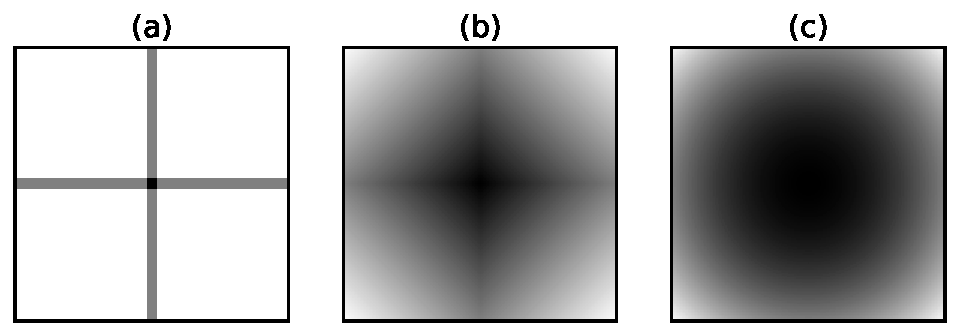
\includegraphics[width=0.4\textwidth]{fig/losses}
    \caption{\textbf{Comparison of loss metrics:}
        \la depicts the $l_0$ pseudo-norm which assigns the same error to all non-sparse vectors. Finding an optimal solution in $\IR^N$ becomes a combinatorial problem with $O(K^N)$ possible solutions in the case of an underlying binary representation.
        \lb depicts a relaxation of the problem with relaxed constraints.
        Maxima in each row and column of the image are located along the axis, making solutions with one component of high magnitude and one of almost zero more probable.
        \lc depicts $l_2$ as a comparison, with a circular error surface, which is not useful in a CS framework.
    }
\label{fig:losses}
\end{figure}

Apart from finding good solutions in terms of a reconstructed signal, it is important to note that the design of $\Measure$ is of great importance within the CS framework.
In a settings where $\Measure$ takes the form of a linear function, a solution to $y = \Measure x$ can only be found if $\Measure$ fulfills the null space property \cite{Donoho2006}.

In many theoretical considerations, the components of the measurement matrix are interpreted as \iid Gaussian random variables.
Given that condition, the probability that $\Measure$ fulfills the restricted isometry property, \ie that it is possible to reconstruct $x$, is very high \cite{Donoho2006}.

Another, probably more practical method is to find a good design for the measurement matrix adapted to the problem.
This can be done by machine learning algorithms that are presented samples from the target domain.
In some problems, this may not be possible (because no training data exists beforehand).
However, in the acquisition of images and audio signals, this technique can be used.

To measure the quality of reconstruction of a CS algorithm, the \abbr{peak signal-to-noise ratio}{PSNR} is used.
It is derived from the \abbr{mean squared error}{MSE} between the original image $x$ and its reconstruction $\hx$.
Assuming $x$ and $\hx$ represent image pixels in the range $[0, 1]$ where $1$ corresponds to white, the PSNR is defined as 

\begin{align}
    \text{PSNR}(x, \hx) &= - 10 \log_{10} \|x - \hx\|_{2}.  \label{eq:psnr}
\end{align}

For comparison with the later experiments, PSNR for a simple DCT based image compression is depicted in \autoref{fig:dct}.
In case of color images, the overall PSNR is computed by averaging the PSNRs of the individual color channels.

\subsection{Sparsity bases for real-world data}

Wavelet transformations can be applied either to the full image or only to distinct patches within the image, as for instance used in JPEG compression.
In the following, the image size will be assumed to be $N \times N$.
In general, a wavelet transformation using the basis $\Basis$ allows to transform input patches from the domain of spatial locations to the domain of spatial frequencies.
The first will be denoted using $n_1, \dots, n_\dims$ while the latter will be denoted using $k_1, \dots, k_\dims$.

Having introduced the necessary semantics, the operation is carried out over an arbitrary number of dimensions $\dims$ using

\begin{equation}
s_{k_1, \dots, k_\dims} = C \sum_{n_1, \dots, k_\dims}
								x_{n_1,\dots,n_\dims}
								\basis_{n_1,\dots,n_\dims}^{(k_1,\dots,k_\dims)}
\label{eq:wavelet-transform}
\end{equation}

The inverse transformation can be performed using the same basis functions and is given by

\begin{equation}
x_{n_1, \dots, n_\dims} = C' \sum_{k_1, \dots, k_\dims}
								s_{k_1,\dots,k_\dims}
								\basis_{n_1,\dots,n_\dims}^{(k_1,\dots,k_\dims)}.
\end{equation}

where $C$ and $C'$ are constants to ensure that applying the transformation twice results in an exact reconstruction of the original signal and depend on the transformation.

Regarding the \abbr{Discrete Cosine Transformation}{DCT}, the basis components for the case of $\dims=1$ are given by

\begin{equation}
\basis_n^{(k)} = \cos \left( \frac{\pi}{N} (n+\frac{1}{2}) k \right).
\end{equation}

For the also commonly used \abbr{Discrete Fourier Transformation}{DFT}, the basis components are given by

\begin{equation}
\basis_{n}^{(k)} = \exp \left( - \frac{2 \pi i}{N} kn \right).
\end{equation}

Using those one-dimensional coefficients, extension to multiple dimensions is straightforward by a superposition according to

\begin{equation}
\basis_{n_1, \dots, n_\dims}^{(k_1, \dots, k_\dims)} = 
	\prod_{i=1}^{\dims} \basis_{n_i}^{(k_i)}.
\end{equation}

For the case of two dimensions, which is interesting in image processing, a visualization of the filter coefficients is given in \autoref{fig:filter-coeffs}.


\begin{figure}
\begin{center}
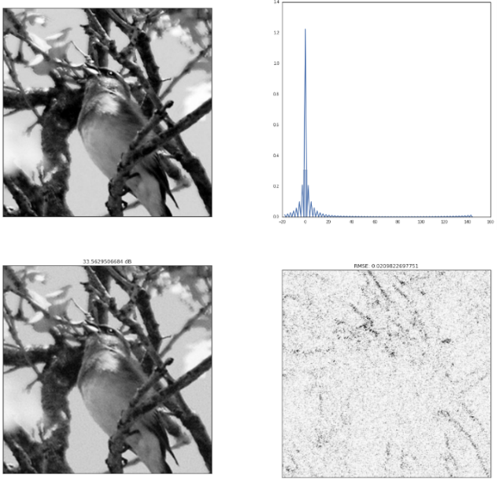
\includegraphics[width=0.4\textwidth]{fig/dct}
\end{center}
    \caption{\textbf{DCT Compression:}
        Demonstration of image compression by using DCT components with highest magnitude.
        Used for comparison with AE approaches.
        $\frac{M}{N} = 0.25$
        }
\label{fig:dct}
\end{figure}

\begin{figure}
\begin{tabular}{cc}
\subfloat[DCT ($8 \times 8$)]{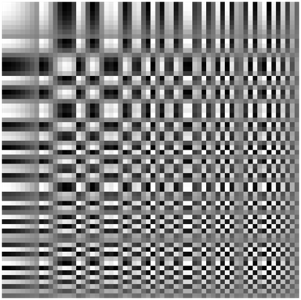
\includegraphics[width = 1.5in]{fig/weights-dct}} &
\subfloat[DFT ($8 \times 8$)]{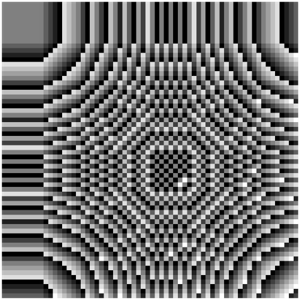
\includegraphics[width = 1.5in]{fig/weights-dft}}\\
\subfloat[GoogLeNet ($7 \times 7$)]{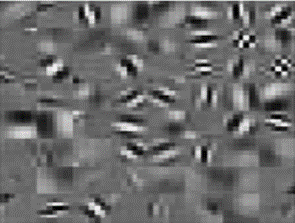
\includegraphics[width = 1.5in]{fig/weights-googlenet}} &
\subfloat[VGGnet ($5 \times 5$)]{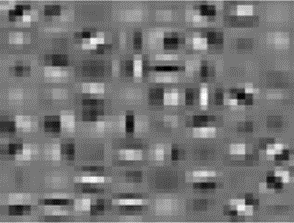
\includegraphics[width = 1.5in]{fig/weights-vgg}}\\
\end{tabular}
\caption{\textbf{Visualization of different possible sparsity transformations:}
	\la and \lb depict the coefficients of wavelet transformations while \lc and \ld depict filters purely learned from data in the first convolutional layers of a neural network.
	The filter weights were obtained by the popular VGGnet architecture by \cite{Simonyan14} and the GoogLeNet architecture by \cite{Szegedy15}.
	It can be seen that the learned filters resemble mathematically motivated filters for wavelet transforms, which motivates the use of neural networks for learning of the sparsity transformation.}
	\label{fig:filter-coeffs}
\end{figure}

\subsection{Deep Learning}

\abbr{Deep learning}{DL} is an emerging field in data science and especially computer vision since the progress made in the \abbr{ImageNet Large Scale Visual Recognition Challenge}{ILSVRC} 2012, where the deep learning model by \cite{Krizhevsky2012} achieved a relative improvement in performance by 50 percent.
Applications of DL to compressive sensing have been presented in \cite{Mousavi2015} and \cite{Palangi2015}.

In DL, neural networks with many layers of representations are used to transform a signal into a compact representation, either for the use in generative models or for classification tasks.
In this review, focus will be on unsupervised learning methods.

Given a random variable $X$ with an unknown underlying distribution modeled by the density function $q(x)$, a dataset $\mathcal X$ with samples drawn from $q(x)$ is provided.
The goal in unsupervised learning is to find a density function $p(x|\mathcal X)$.
This is usually done by fixing the number of possible functions to a certain class of models which can be described by a weight vector $\theta$.

Different approaches exist: In \abbr{Restricted Boltzmann Machines}{RBM}, the distribution of $X$ is modeled directly using an energy based graphical model, yielding

\begin{equation}
    p(x) = \frac{1}{Z} \exp(- F(x)).
\end{equation}

Every state of the model is assigned an energy $E(x, h) = f(x,h,\theta)$ which can be marginalized to obtain the free energy $F(x) = - \log \sum_h \exp (- E(x, h))$.
Before pre-trained models on large datasets and advanced initialization schemes became available, RBMs provided a convenient way to find initial weights for deep networks \cite{Hinton2006a}.

As shown by \cite{Bengio2007}, the (computationally expensive) training procedure of RBMs can be approximated by \abbrpl{Autoencoder}{AE}.
AEs model a distribution $p(\hat x | c(x) )$ to reconstruct the signal $x$ from a code $c$.

Given a dataset $\ds$ with training samples, the predictive distribution of a previously unseen example $x$ is given as

\begin{equation}
    p(\hat x | x, \ds) = \int_{f} p(\hat x | f, x) p(f | x, \ds) df \label{eq:predictive}
\end{equation}

where $f$ denotes a possible function which can be modeled by the AE.
Usually, AEs are composed of convolutional or fully connected layers with a fixed structure.
The exact properties of the model are given by a set of adaptable weights which are summarized as a single tensor $\theta$ which parametrizes $f$.
\eqref{eq:predictive} then becomes

\begin{equation}
    p(\hat x | x, \ds) = \int_{\theta} p(\hat x | f_\theta(x)) p(\theta | \ds) d\theta .
\end{equation}

The posterior $p(\hat x | f_\theta(x))$ is chosen to be a normal distribution of \iid pixels with the mean given by $f_\theta(x)$.
Thus, $p(\hat x | f_\theta(x)) = \normal (\hat x | \mu=f_\theta(x), \Sigma=I)$.
Other choices are possible, in particular the variance could also be modeled, which is used in Variational AEs \cite{Kingma2014}.

The second distribution $p(\theta | \ds)$ describes the likelihood for each weight vector and is optimized during training. This is why the distribution is independent from the current example $x$. 
For a denoising AE, it is assumed that the input vector is not exactly equal to the desired output vector and contains noise.
Consequently, the dataset $\ds$ consists of pairs of corrupted images and the desired denoised reconstruction, \ie $\ds = \{(\tx^{(1)}, x^{(1)}) \dots (\tx^{(N)}, x^{(N)})\}$.

Iterating over the samples within the dataset yields

\begin{equation}
    p(\theta | \ds) = \frac{1}{Z} p(\theta)
    		\prod_{l = 1}^{N} p(x^{(l)} | f_\theta (\tx^{(l)}))
\end{equation}

where $Z=p(\ds)$ is a normalizing constant, $p(\theta)$ defines the prior distribution over the weights and $p(x^{(l)} | f_\theta (\tx^{(l)}))$ is the posterior of reconstructing a sample from the training data using the current weight vector.
This distribution is optimized during training, in order to find the weight vector which best explains the dataset in terms of its likelihood.
Maximizing $p(\theta | \ds)$ is equivalent to minimizing the negative log-likelihood.
Assuming a zero mean Gaussian prior distribution $p(\theta)$ with precision $1/\sigma^2 = \lambda$ and a Gaussian posterior with unit variance and mean $f_\theta(\tx^{(l)})$ as discussed before yields

\begin{align}
    &-\log p(\theta | \ds) \\
    &=   \log{Z} - \log p(\theta) - \sum_{l = 1}^{N} \log p(x^{(l)} | f_\theta(\tx^{(l)}))
\end{align}

where $Z = p(\ds) < 1$ and thus $\log Z < 0$.
Furthermore,

\begin{equation}
    - \log \normal (x | \mu, \lambda=\sigma^2) = \frac{1}{2} \frac{\log 2 \pi}{\lambda} + \lambda (x - \mu)^2 .
\end{equation}

Since all densities were assumed to be Gaussian densities, the upper bound on the negative log a-priori is therefore given as

\begin{align}
    &- \log p(\theta) - \sum_{l = 1}^{N} \log p(x^{(l)} | \theta \tx^{(l)}) \\
    &\lambda \|\theta\|_2  + \sum_{l = 1}^{N} \|x^{(l)} - f_\theta(\tx^{(l)})\|_2 . \label{eq:loss}
\end{align}

The first term acts as a regularizer incorporating the prior for the weights, while summing over all training examples corresponds to the actual learning process.
This function is optimized using \abbr{stochastic gradient descent}{SGD} with \abbr{backpropagation}{BP}.
During training, the gradient of \eqref{eq:loss} \wrt the weights $\theta$ is optimized.

It should be noted that this directly optimizes the PSNR defined in \eqref{eq:psnr} and therefore meets the defined target within the CS framework.

\section{Compressive Sensing with Autoencoders}

\begin{figure}
\begin{center}
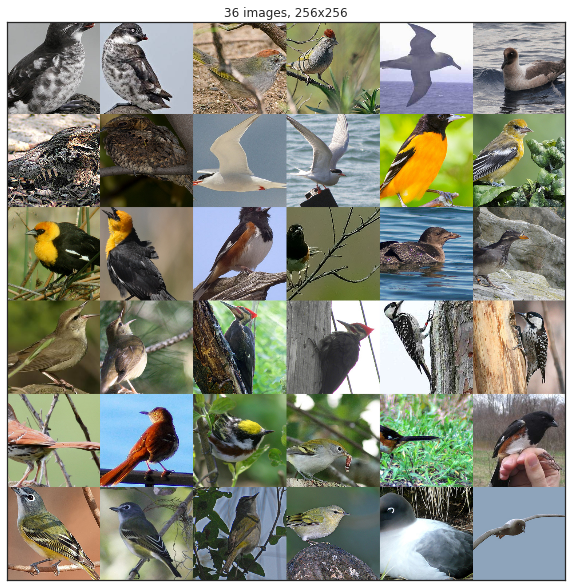
\includegraphics[width=0.4\textwidth]{fig/birds}
\end{center}
   \caption{
       \textbf{Samples from the Caltech Birds 2011 dataset used in the experiments:}
       The dataset consists of more than 200 different species of birds, usually with an order of 10-100 sample images per class. For the experiments, random species were selected and no more than 5-10 images of the same species were used.
   }
\label{fig:dataset}
\end{figure}

In \cite{Mousavi2015}, the authors use a stacked denoising AE with an alternating structure of four layers plus an additional layer in case the measurement process should be adapted by the neural network directly.
The traditional formulation of AEs was used, \ie specifying the applied learned transition between two subsequent layers as an affine transformation $Wx+b$ followed by a sigmoid nonlinearity of the form $\sigma(x) = 1/(1+e^{-x})$.
To apply the model to a full scale image, the authors separated it into patches of size $32 \times 32$ including an overlap during test time to reduce noise.
The network was then trained on images from the ImageNet dataset using BP.
In addition, pre-training using RBMs was used to find a good initialization of the weights as well as inferring the energy function of the AE as proposed by \cite{Kamyshanska2015}.

Two different models are discussed for solving two relevant questions within the CS framework:
In the first model, a measurement vector derived from the linear transformation $y = \Measure x$ is considered, which is directly fed into the AE.
It is transformed in four alternating layers covered by the functions

\begin{align}
    x_{h_1} &= \sigma (W_1 y + b_1),       \label{eq:firstlayer} \\
    x_{h_2} &= \sigma (W_2 x_{h_1} + b_2), \label{eq:secondlayer} \\
    \hx     &= \sigma (W_3 x_{h_2} + b_3). \label{eq:thirdlayer} 
\end{align}

In a second model, the AE is also used to directly infer a good choice for the measurement function.
This is done by inserting an additional layer for the transition between $x$ and $y$, \ie the measurement function is represented as a layer of the network.
Assuming $\xi$ denotes a nonlinearity (potentially again a sigmoid function), this layer is covered by 

\begin{equation}
    y = \xi (\Measure x + b).
\end{equation}

\subsection{Introducing convolutions}

The authors in \cite{Mousavi2015} note the need for extracting patches before training this kind of model.
This problem is merely caused by the choice of using a fully connected architecture.
In many computer vision problems, it is therefore more convenient to use a convolutional network instead of a fully connected architecture.
This allows an application to process images of arbitrarily large dimensions, provided the used hardware is capable of storing all intermediate feature representations.

In a convolutional neural network, dot products between weights and input units as denoted in Equations \eqref{eq:firstlayer}-\eqref{eq:thirdlayer} are replaced by a convolution of the input with a kernel matrix.
For dealing with images, 2-D discrete convolutions are used.
Considering an input tensor $x \in \IR^{C \times N \times N}$ and a kernel tensor $W \in \IR^{K \times C \times M \times M}$ where $C$ denotes the number of input channels (\eg RGB channels in an image), $K$ the number of output channels and $x$ representing an image of size $N \times N$, computation of $h$ is done by

\begin{equation}
    h^{(k)} = \sum_c x^{(c)} * W^{(k, c)}
\end{equation}

where $a * b$ is discrete 2-D convolution with

\begin{equation}
    (a * b)_{x,y} = \sum_{u, v} a_{x-u, y-v} b_{u, v} \quad \forall x, y .
\end{equation}

Densely connected architectures with a kernel can always be regarded as a convolutional layer: When $W_\text{dense} \in \IR^{M^2 \times K}$ is applied to patches of size $M \times M$ with $K$ features computed by the layer, it can be \emph{reshaped} to match the formulation $\IR^{K \times C \times M \times M}$ from above.
Intuitively, this is directly equivalent to splitting the image into several patches at a stride\footnote{Difference between the center of the patches.} of 1 and application of the dense operation to each of those patches.
The stride can also be adjusted: An architecture as proposed by \cite{Mousavi2015} can be formulated as a convolutional AE with kernels of size $32 \times 32$ at a stride of 16, resulting in a smoother reconstruction of the image. 

As results by \cite{Szegedy15} and \cite{Simonyan14} from recent deep learning research suggest, it is preferable to do this in a hierarchical manner.
The VGG architecture \cite{Simonyan14} is commonly used in this context.
In addition, sigmoid units are omitted and replaced by \abbrpl{Rectified Linear Unit}{ReLU} which generally provide a greater expressibility of the model with a lowered computational complexity \cite{Nair2010}.

It is composed of computational blocks of $3 \times 3$ convolutional filters followed by pooling layers with a stride of $2$.
After five pooling operations, the effective image size is reduced by a factor of $1/32$ and the resulting units will incorporate the mentioned receptive field.
The ReLU operation is given by $\max(\cdot, 0)$.


\section{Experiments}

\begin{figure*}
\begin{center}
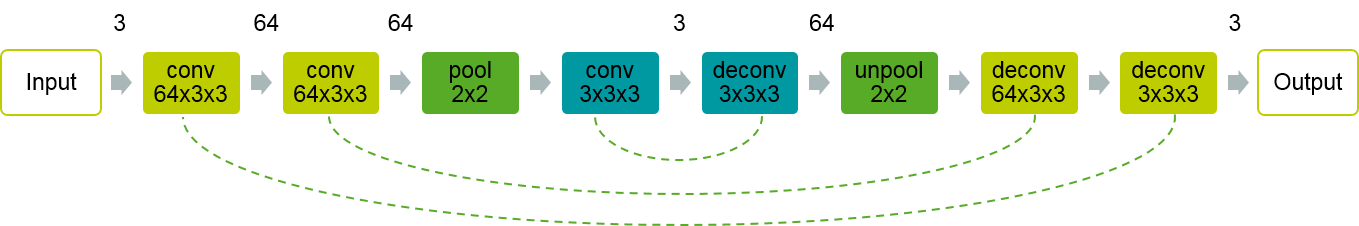
\includegraphics[width=\textwidth]{fig/vgg-architecture}
\end{center}
   \caption{
       \textbf{The proposed VGG-like architecture:}
       The input image is first transformed into an overcomplete and likely sparse representation by application of two convolutional blocks as in the original VGG architecture.
       These blocks were initialized using the VGG weights pre-trained on the ImageNet dataset.
       The resulting filter map undergoes spatial pooling, reducing the filter map size by a factor of 4.
       Afterwards, another convolution compresses the feature representation and outputs filter maps spatially reduced by a factor of 4, while the number of feature maps is 3.
       Overall, after this bottleneck operation, the measurement vector with $\frac{M}{N} = 0.25$ is obtained.
       In the backward pass, deconvolution with tied weights and unpooling using the stored pooling indices upsamples the measurement vector and is used for reconstruction of the image.
       Note that normalization layers were omitted in the figure.
   }
\label{fig:network-structure}
\end{figure*}

\begin{figure*}
\begin{center}
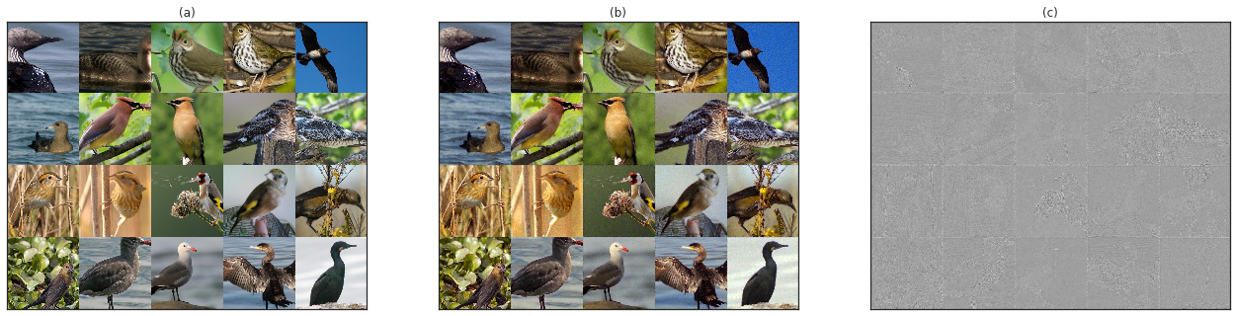
\includegraphics[width=0.9\textwidth]{fig/vgg-ae-rgb-2}
\end{center}
   \caption{
       \textbf{Image Reconstruction with pre-trained AE:}
       \la depicts original images fed into the network.
       Those are compressed by a factor of $\frac{M}{N} = 0.25$ using a learnable, nonlinear measurement function.
       \lc depicts the residuum, averaged over all color channels.
       Average PSNR over all images and color channels was 25.3 dB.
   }
\label{fig:reconstruction}
\end{figure*}

Different experimental setups using convolutional architectures instead of fully connected networks are possible.
Three possible model configurations are:

\begin{itemize}
    \item 	Autoencoder as in \cite{Mousavi2015} interpreted as a convolutional architecture.
        	The first layer performs a valid convolution with a $32 \times 32$ filter at stride 16,
        	resulting in an overlap.
    \item 	Using the first block of a VGG network, \ie the first two convolutional layers as well as the first
    		pooling layer. The image is convolved with an effective filter size of $5 \times 5$ for two times.
    		After pooling, the image size is reduced by a factor of $4$ in the spatial dimensions, however the
    		number of feature maps increases considerably (from 3 to 64). Therefore, the resulting representation
    		is compressed by another convolutional layer which outputs only three feature maps.
    \item 	A similar scheme can be applied to a full VGGnet using all five blocks proposed by \cite{Simonyan14}.
    		After the fifth network block, spatial resolution is reduced by a factor of 32 in each dimension, while
    		the number of feature maps has grown to 512. Thus, an input block of size $32 \times 32$ with three channels
    		is already compressed by a factor of $1/6$.
\end{itemize}

For the remainder of this report, the second architecture will be further considered.
Since convolution and fully-connected layers applied to image patches are mathematically identical operations, the first architecture is unlikely to improve on the results of \cite{Mousavi2015}.
The last rather complex approach with a full scale VGGnet applied to the CS problem will be left to open research, since the detailed analysis of the network would exceed the scope of this report.

\subsection{Review}
The authors in \cite{Mousavi2015} have shown that the usage of DL in the CS framework helps to overcome several problems, including the design of the measurement matrix, knowledge of the sparse domain underlying the image data and long reconstruction time due to iterative algorithms.

Especially the latter aspect can be regarded as a huge improvement, since the overall reconstruction performance of the proposed model ranks among other popular CS algorithms, while cutting reconstruction time by a factor of 100 to 1000.

DL models are superior to iterative algorithms since they only have to be fitted to the data \emph{once}.
After finding a good configuration for the sparsity and measurement matrices, direct inference is possible without the need of iteratively improving the reconstruction result.

\subsection{Extensions}

The detailed structure of the extended AE network is given in \autoref{fig:network-structure}.
Hyperparameters for training the network are the learning rate $\eta$ and the momentum $\epsilon$ used in stochastic gradient descent as well as the size of the intermediate convolutional layer.
In order to reduce the total number of parameters, tied weights were used between the encoder's convolutional layers and the decoder's deconvolutional layers.
In the context of convolutional AEs, tied weights are realized by vertically and horizontally flipping the weight matrices.

The momentum was fixed to $\epsilon = 0.9$ according to the values commonly found in DL literature \cite{Simonyan14, Szegedy15}.
The learning rate was determined by a line search starting at $10^{-1}$ by watching the decrease in training error in the first epochs of training.
It was fixed to $10^{-3}$ for the final setup.
Another line search was performed on the size of filters in the bottleneck module.
With a small filter size of $3 \times 3$, the network was not able to capture larger texture element in the image, which resulted in noisy reconstructions.
No significant difference between $5 \times 5$ and $7 \times 7$ convolutions could be found, so that the first one was chosen due to increased inference speed and a reduced number of parameters.
In principle, this convolutional layer could also be split up into a stack of subsequent $3 \times 3$ convolutions to reduce the parameter size even more.

As the VGG network was not originally designed to perform reconstruction of images, the convolutional filters have to be normalized to ensure proper output scales.
Effectively, this can be interpreted as finding $C$ in Equation \eqref{eq:wavelet-transform}.
The block's weights are used in a convolutional forward pass with valid convolutions, followed by a pooling layer.
In the bottleneck module in the middle of the network, \abbr{Batch Normalization}{BN} is used to normalize the propagated signals and ensure a more stable training procedure.
After the network's output layer, another BN module is inserted to act as a linear transformation for exact fitting of the colorspace.
This layer prevents that convolutional filters have to be adapted to very high values, which would slow down the whole training procedure.

The model is deployed in Theano \cite{Bergstra2010} using Lasagne \cite{Dieleman2015} as a high level framework on top.
The performance is tested using images from the Caltech-UCSD Birds-200-2011 Dataset \cite{Wah2011}.
During training, images are randomly sampled from the training set.
About 4000 images were used for training the final model.
The final model achieves a PSNR of over 25 dB on this dataset.
Some example reconstructions are depicted in \autoref{fig:reconstruction}.


\section{Conclusion and Future Work}

Using DL techniques in CS provides a convenient way to reduce reconstruction times within the framework and enables to learn sparsity transformations as well as measurement matrices purely learned from the data.
This report further investigated the work of \cite{Mousavi2015} and extended the proposed framework by introducing convolutional network layers for efficient image processing regardless of input image shape.
It was shown that existing models such as the VGGnet are suitable for use in a transfer learning setting:
Inspired by the architecture of VGGnets, a convolutional AE was deployed and trained for automated adaption of the measurement matrix as well as image reconstruction.

Further research in this field may include the use of full scale deep learning models and more sophisticated model structures.
In this context, this report introduced a proof-of-concept architecture for CS with a DL model.


{\small
\bibliographystyle{ieee}
\bibliography{references}
}

\end{document}
